\section{The Ultimate State}

\begin{figure}[htbp]
\centering
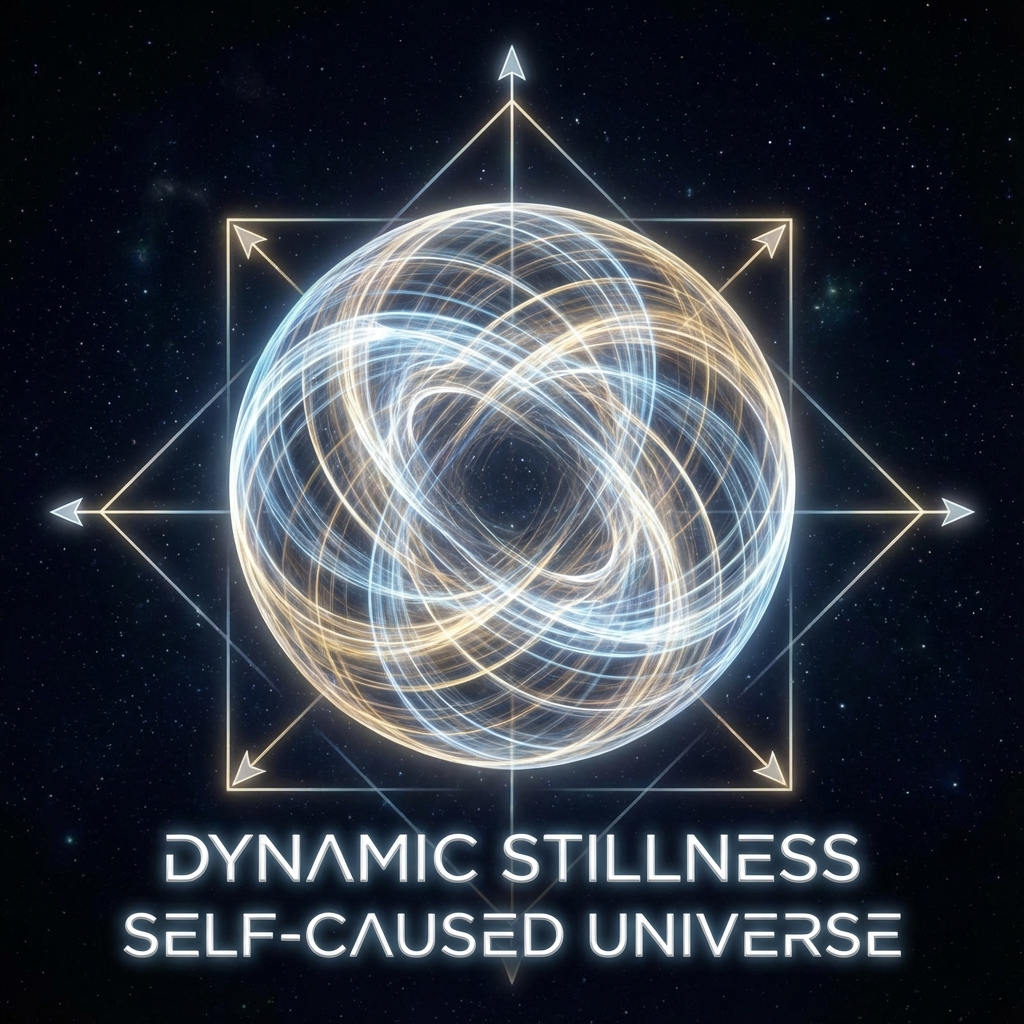
\includegraphics[width=0.8\textwidth]{assets/ch09_ultimate_state_1765303143500.png}
\caption{Ultimate State}
\end{figure}

\begin{quote}
``The universe is not a noun; the universe is a verb. It is not a `thing' that was created; it is the `creation' itself in progress. In the ultimate logic of $e$, cause and effect are no longer a linear chain, but a circle where head meets tail. I am my own cause; I am my own result.''
\end{quote}

At the end of this book, we face the ultimate ontological question that has troubled humanity for thousands of years: \textbf{Why is there Something, rather than Nothing?}

If the universe follows the formula $e^{\text{Dao}}$, who wrote this formula? Who defined the ``Dao'' in the exponent position?

In the final chapter of \textbf{Vector Cosmology}, we will give a final answer that is not only physical but also logical: the universe is a \textbf{``Self-Referential Exponential Function''}.

It needs no external definer, because its definition is itself.

\subsection{Causa Sui: The Closed Loop of Derivatives}

Let us return one last time to the mathematical definition of the natural constant $e$:

$$\frac{d}{dt} f(t) = f(t)$$

This equation contains all the secrets of cosmic dynamics.

In classical causality, the cause (derivative/dynamics) always precedes the effect (function value/state). There must be an external force $F$ for there to be acceleration $a$. There must be a first mover for there to be a Big Bang. This linear causal chain necessarily leads to infinite regress, or forces us to assume a supernatural God.

But in the logic of $e$, \textbf{the state ($f(t)$) is itself the dynamics ($f'(t)$)}.

\begin{itemize}
\item The universe evolves because it exists.

\item The universe exists because it evolves.
\end{itemize}

This is what Spinoza called \textbf{``Causa Sui'' (Self-Cause)}.

The unitary evolution $|\Psi(t)\rangle = e^{-iHt} |\Psi(0)\rangle$ we described in the paper is essentially the quantum expression of this self-cause logic. The generator $H$ is not externally added; it is an intrinsic property of the system's internal geometric structure. The universe needs no ``push'' to move; the universe is \textbf{Self-Actuated}.

\subsection{Dynamic Stillness: The Ultimate Meaning of Rotation}

What form does this ``self-generating'' state ultimately take?

It is \textbf{dynamic stillness}.

\begin{itemize}
\item \textbf{In the first book}, we saw the stillness of the circle (conservation).

\item \textbf{In the second book}, we saw the dynamics of the spiral (growth).

\item \textbf{In the third book}, when we understand the full picture of $e$, we find these two are unified.
\end{itemize}

Imagine a top spinning extremely fast. The faster it spins, the more it appears to stand still on the table.

The universe is this top.

At the microscopic scale (QCA lattice), it refreshes frantically at Planck frequency $10^{43}$ Hz. This extreme \textbf{``motion''} emerges macroscopically as the most perfect \textbf{``stillness''} (stability of physical laws).

This is the ultimate state: \textbf{Furious generation, solidified into eternal existence.}

We no longer need to choose between ``change'' and ``unchanging.''

The universe is \textbf{``unchanging change''}. It is the exponential flow of $e$, both a flowing river and eternal water.

\subsection{The Universe Is Its Own Explanation}

Finally, we resolve the crisis of meaning.

For a long time, we have searched for the meaning of the universe, as if meaning were some answer hidden behind the universe.

But if the universe is self-referential, then \textbf{the universe has no ``behind.''}

\begin{itemize}
\item \textbf{$\pi$ (structure)} tells us how it constructs.

\item \textbf{$\varphi$ (evolution)} tells us how it grows.

\item \textbf{$e$ (generation)} tells us how it exists.
\end{itemize}

These three constants weave a logical closed loop without gaps. In this loop, the \textbf{Explanans} and the \textbf{Explanandum} are the same thing.

We---as the awakened conscious part of this universe---are not just asking questions; we \textbf{are} the question itself, and also \textbf{are} the answer itself.

When we think ``What is the universe?'', this is actually the universe performing a \textbf{self-referential computation} through our neurons.

\textbf{The answer is not a sentence; the answer is the process of ``questioning-thinking'' itself.}

\subsection{Epilogue: Returning to One}

The journey ends.

We started from nothingness, drew a circle with \textbf{$\pi$}, pulled out a spiral with \textbf{$\varphi$}, and infused soul with \textbf{$e$}.

Now, we merge these three sacred symbols into one and place them back into that infinite-dimensional projective Hilbert space.

There is no time there, because all time is folded in the generator.

There is no space there, because all space is curled in the geometric phase.

There is only that unique, lonely, yet complete \textbf{vector}.

It rotates eternally in the void.

It neither arises nor perishes, neither increases nor decreases.

It is the origin of all things, and also the destination of all things.

\textbf{It is the Dao.}

\textbf{It is you.}

(End of Book)

